\documentclass[12pt,a4paper,oneside,english,brazil]{article}
  \usepackage[abnt-emphasize=bf,abnt-and-type=e,alf]{abntex2cite}
  \usepackage{times}
  \usepackage[left=3cm, top=3cm, right=2cm, bottom=2cm]{geometry}
  \renewcommand{\baselinestretch}{1.5}
  \usepackage{indentfirst}
  \usepackage{graphicx}
  \graphicspath{ {./images/} }
  \renewcommand{\figurename}{\textbf{Fig.}}
  \setlength{\parskip}{0.2cm}

  \usepackage{listingsutf8}
\usepackage{listings}
\usepackage{courier}

\usepackage{xcolor}
\definecolor{lightgray}{rgb}{0.95,0.95,0.95}
\definecolor{codegray}{rgb}{0.5,0.5,0.5}

\lstdefinestyle{meuestilo}{
	inputencoding=utf8/latin1,
  backgroundcolor=\color{lightgray},
	numberstyle=\tiny\color{codegray},
	basicstyle=\ttfamily\footnotesize,
	breakatwhitespace=false,
	breaklines=true,
	captionpos=b,
	keepspaces=true,
	numbers=left,
	numbersep=7pt,
	showspaces=false,
	showstringspaces=false,
	showtabs=false,
	tabsize=2
}

\lstset{style=meuestilo}


    \title{
      \textbf{Hive} \\
      \large um estudo de caso do uso de desenvolvimento guiado por testes para
      alcançar uma arquitetura limpa na construção de um jogo para internet com
      múltiplos competidores
    }
    \author{Hudson Ferreira Leite}
    \date{2021}

\begin{document}
  \maketitle

  % % apenas se o número de figuras exceder 10
  % \clearpage

  %   \renewcommand{\listfigurename}{Lista de Figuras}

  %     \listoffigures

  \clearpage

  \section{Introdução}

    Desenvolver software sempre foi uma atividadade complexa, que pode,
    facilmente,  apresentar desafios das mais diveras naturezas: agendamento;
    má-definição de  requisitos - funcionais ou não; sub - ou super -
    dimensionamento de recursos; não-escalabilidade; etc.

    Negligenciar esse amálgama de possibilidades é um erro comum, e até
    esperado, de profissionais pouco experimentados, mas, não raro,
    encontram-se exemplares com bastante quilometragem de carreira a
    cometê-los.

    O Standish Group demostra, em seu \emph{Chaos Report}\cite{ChaosReport2015},
    que quanto maior o projeto maior é a chance de falha. O mesmo relatório, no
    entanto, aponta alguns caminhos a seguir para encontrar sucesso: \emph{uma
    arquitetura padrão} e \emph{um processo ágil}.

    Ao mencionar agilidade é possível inferir que a capacidade de adaptação é
    uma  necessidade fundamental para o bom andamento, princípio defendido desde
    a  primeira hora por este tipo de metodologia \cite{ManifestoAgil2001}.

    Quanto à  arquitetura, faz-se evidente que, utilizar um padrão é uma decisão
    que  pode poupar longas, e pouco frutíferas, discursões sobre assuntos já
    consolidados.

  \section{Testes}

    Se estabelecermos um marco na história da programação como sendo a parceiria
    entre a matemática londrina Ada Lovelace, e o, também, matemático londrino
    Charles Babbage\footnote{\cite{Huskey1980}}, pode-se dizer que essa
    disciplina possui mais de 180 anos, e com ela dois grande problemas: 1.
    especificar o comportamento de um software; 2. garantir que um software não
    possua defeitos.

    No primeiro, por mais avanços que se tenha feito no campo da engenharia de
    software, essa é, ainda, uma área bastante desafiadora. No último, Disjkstra
    estatuiu que \emph{testes mostram a presença, não a ausência de defeitos}
    \cite[p. 16]{Nato1969}.

    Daí a necessidade de se testar \cite[p. xxix-xxx]{Mezaros2007}: 1.
    paulatinamente construir conhecimento através da retroalimentação de
    hipóteses; 2. exaustivamente chegar a um ponto onde não é possível provar a
    presença de defeitos.

    Testes, segundo os métodos tradicionais de desenvolvimento, são feitos em
    etapa posterior a sua construção, para \emph{medir qualidade}. Uma abordagem
    diferente daquela que deseja \emph{construir qualidade}\footnote{\cite[p. 7]
    {FarcicGarcia2015}}. Isso reverbera de maneira
    distinta \emph{quem} os executa: uma equipe independente daquela que
    construiu o software ou o próprio desenvolvedor?


    \subsection{Desenvolvimento Guiado por Testes (TDD)}

      Dentre as práticas que sustentam os métodos ágeis, o uso de testes, como
      uma atividade de suporte às demais, é um fato consolidado. Mas a abordagem
      do TDD, também conhecida por \emph{testar primeiro} é ainda mais difundida
      nesse  meio.

      É bem corriqueiro ver profissionais se referindo à  técnica como
      "desenvolvimento orientado \emph{a} testes", dando a entender que seu
      objetivo é produzir um código que seja testável, o que é, claramente, uma
      consequência do seu uso. Ao passo que uma tradução que melhor exprime o
      conceito é "desenvolvimento orientado {por} testes".

      A ideia é extremamente simples \cite[p.1]{FreemanPryce2009}: \emph{escrever um
      teste para um código que ainda não existente}, sumariamente falando, mas
      de maneira mais completa, trata-se de um ciclo de três etapas (Fig.
      \ref{fig:ciclotdd}): red,  escreva um teste para o qual não existe uma
      implementação, portanto, não deve estar passando nesse momento; green, faça
      o mesmo passar, escrevendo o código da funcionalidade pretendida; refactor,
      remova duplicações e melhore a legibilidade.

      \begin{center}
        \begin{figure}[h]
          \centering
          \caption{Ciclo TDD}
          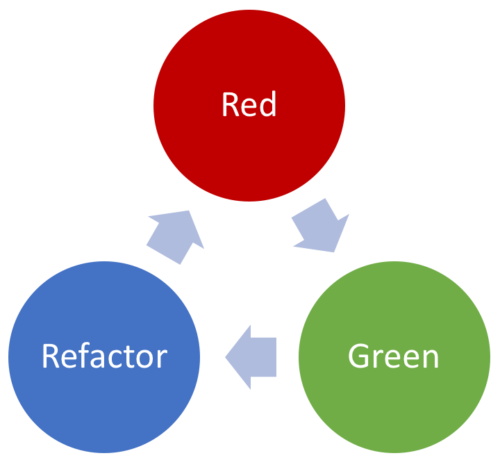
\includegraphics[width=3cm]{ciclo-tdd}
          \label{fig:ciclotdd}
        \end{figure}
        Fonte: Blog da Knowledge21\footnote{\cite{Ferreira2018}}
      \end{center}

      Essa postura realoca o papel dos testes de uma atividade meramente focada
      em descobrir defeitos para uma posição centrada na experiência do
      usuário, ao  \emph{orientar} a desenvolvedora no entendimento das reais
      necessidades dos primeiros, através de um processo dialético de construção
      de conhecimento \footnote{\citeonline[p.28]{Oliveira1992} sugere, ao
      analisar Vygotsky e o processo de formação de conceitos, que os últimos
      são construções culturais, internalizadas pelos indivíduos ao longo do seu
      processo de desenvolvimento.}.

      Isso explica porque \citeonline[p.3-5]{FreemanPryce2009} colocam a prática
      como fundamentada em três pilares: 1. aprendizagem; 2. retroalimentação;
      e, 3. suporte a mudança.


  \section{Arquitetura de Software}

    A engenharia de software, enquanto disciplina da ciência dos
    computadores, recebe o seu primeiro nome graças a uma série de
    propriedades que lhe são comuns com sua "aparentada" e seu
    sobrenome, em função de características que lhe são peculiares.

    Tal fenômeno, bastante comum nessa área do conhecimento, explica a
    denominação da chamada \emph{arquitetura de software} que, na ausência de
    uma expressão mais apropriada, toma emprestado a alcunha para conceituar uma
    abordagem com alto nível de abstração, que a "matéria dos dígitos binários"
    exige.

    Vejamos a definição do verbete inicial da locução: \emph{1. arte de
    projetar, construir, decorar e oraganizar os espaços de uma edificação; 2.
    obras arquitetônicas que caracterizam uma época ou povo \footnote{\cite[p.
    81]{Kury2007}}}.

    Ainda, etimologicamente, a palavra remete à composição grega de \emph{
      ARKHEIN} - que significa \emph{comandar}, em português - com \emph{TEKTON}
    - que, por sua vez, quer dizer \emph{artesão ou construtor}\footnote{\cite{
    Etimologia2019}}.

    Por aproximação, diz tratar-se dos dítames direcionadores de uma determinada
    construção. Ora, não resta dúvida, assim, que arquitetura de software são os
    preceitos orientadores de um sistema computacional.

    \subsection{Arquitetura Limpa}

      Se ao vislumbrar determinada edificação é possível inferir algumas
      características de uma obra, seria possível realizar o mesmo exercício ao
      observar um "programa computacional"?

      A depender da forma como um prédio é arquitetado, é factível realizar
      alterações funcionais sem prejuízo à estrutura, ou, ainda, sem qualquer
      noção do dano que tais modificações podem desencadear.

      Tal qual uma arquitetura, convencional, limpa "grita"\cite[p. 196]{
      Martin2018} qual é a sua motivação - uma casa, uma biblioteca, uma fábrica,
      etc. - uma arquitetura, de software,  limpa diz \emph{o quê é} e \emph{o
      que é possível fazer em seu contexto}.

  \section{Como TDD auxilia na processo de chegada a uma Arquitetura Limpa?}

    É fácil encontrar muitas similaridades entre as arquiteturas citadas, mas
    existe um quesito que pesa a favor da última: software, como o nome sugere,
    soft (em português: flexível, suave) é um bem intangível, cuja construção,
    guardadas as devidas proporções e contextos, não oferece os mesmos riscos,
    por vezes irreparáveis, que a primeira.

    Desenvolvimento orientado por testes privilegia uma conduta que permite
    definir as funções essenciais do sistema, implementá-las da maneira mais
    simplória conhecida e através de sucessivas modificações, amparadas por uma
    rede de proteção que previne regressões, alcançar um modelo que expressa,
    claramente, quais seus objetivos e permite uma evoluçãi sustentável do
    produto.

  \section{O estudo de caso}

    \subsection{O jogo}

    Hive\footnote{Adaptado de \cite{UltraBoardGames2020}.} é um jogo
    abstrato de duelo, tal qual o xadrez, onde os jogadores devem usar seus
    respectivos acervos para cercar o alvo oponente.

    Cada jogador possui onze peças em formato hexagonal de cinco tipos
    distintos, cada tipo sendo representado por um inseto: uma abelha rainha, o
    alvo; duas aranhas; dois besouros; três gafanhotos; e, três formigas.

    Apenas uma ação, das duas possíveis, é permitida aos jogadores executar por
    turno: entrada e movimentação.

    Quando entra em jogo, uma peça deve ser colocada adjacente a uma que já
    está, à exceção daquela colocada no primiero turno do jogo. Ela também não
    deve tocar nenhuma peça adversária, reservada aquela que o faz no segundo
    turno, posto que a regra anterior deve ser atendida.

    A abelha rainha deve entrar, no máximo, até a quarta rodada. Enquanto isso
    não ocorrer, nenhuma peça irmã poderá ser movimentada.

    Os insetos tem movimentações diversas. A abelha rainha, um passo por vez ao
    redor da colméia. As aranhas, três passos ao redor da colméia, sempre na
    mesma direção iniciada. Os besouros, um passo ao redor da colméia ou acima
    dela, e a peça sob o qual ele pousa fica imobilizada até que ele a deixe e,
    para efeito de novas entradas, a posição ocupada assume a cor do mesmo. Os
    gafanhotos, se movimentam sobre a colméia, iniciando de um lado e seguindo
    em linha reta (perpendicular a aresta escolhida) até o lado oposto.
    E,  as formigas, o fazem ao redor da colméia sem limites de passos. Tais
    ações não podem resultar em uma colméia fragmentada, mesmo que o resultado
    seja uma colméia intacta. As movimentações ao redor devem ser de livre
    deslize, não sendo permitido entrar em uma posição onde isso não é possível.

    Finalmente, a abelha rainha é considerada cercada quando todos os seus lados
    estão ocupados por alguma peça em jogo, independente de a quem elas
    pertençam.


    \subsection{O escopo}

      O objetivo é construir uma aplicação web onde um usuário qualquer possa se
      cadastrar para adquirir acesso. Uma vez autenticado o citado pode se
      disponibilizar para uma partida com um adversário aleatório\footnote{
      Poderíamos extender as capacidades do sistema para permitir que um usuário
      escolhesse/convidasse seu adversário para uma partida ou, ainda, criar um
      ranking dos melhores jogadores, mas vamos manter as coisas mais enxutas,
      pois aqui o foco é desenvolver os conceitos e não entregar uma solução
      completa.}.


    \subsection{A solução}

      Primeiramente
      \footnote{Mesmo sendo um jogo com regras, relativamente,
      simples, e uma aplicação com escopo bem limitado, este é um estudo que não
      se encerra em 20 páginas, considerando a quantidade de código que pode vir
      a ser gerada. Também é necessário salientar que o contexto de automatizar
      um processo cujas regras já estão bem definidas apresenta privilégios não
      compartilhados em uma situação mais próxima do real, mas servem bem aos
      critérios didáticos pretendidos.},
      usamos a técnica de \emph{mapeamento de histórias de usuário}\footnote{
      \cite{Patton2014}} para identificar fluxos completos de uso (Fig.
      \ref{fig:fluxogeral}). Essa técnica permite definir todas as histórias que
      o usuário deseja ver implementadas mas, também, aquelas que agregam maior
      valor ao resultado, possibilitando a delimitação de um produto mínimo
      viável (MVP) que atenda às necessidades daquele e, ainda, gerenciem os
      riscos de construir uma solução pormenorizada, antes mesmo de validar
      algumas hipóteses.

      \begin{center}
        \begin{figure}[h]
          \centering
          \caption{Mapeamento de Histórias de Usuário}
          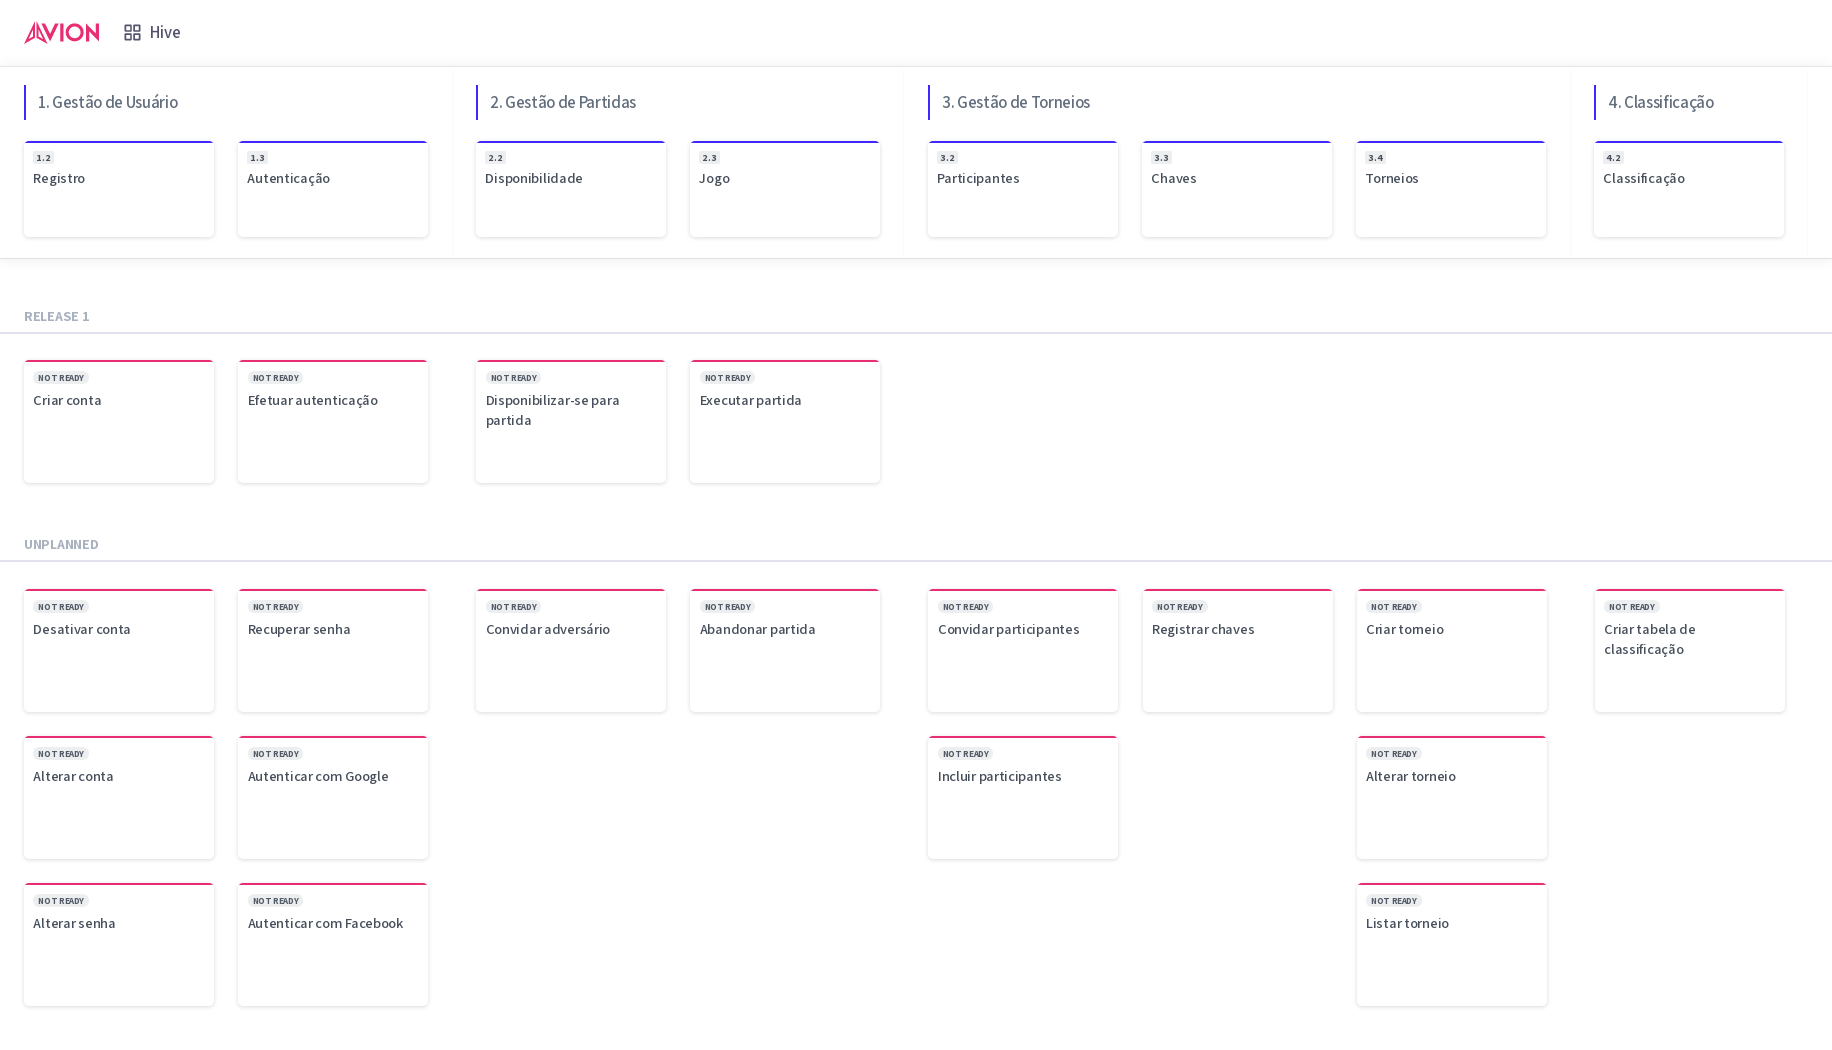
\includegraphics[width=16cm]{user-stories-mapping}
          \label{fig:fluxogeral}
        \end{figure}
        Fonte: Próprio autor\footnote{Criado em "https://app.avion.io"}
      \end{center}

      Assim, podemos perceber que quatro funcionalidades são essenciais para o
      MVP: Criar conta; Efetuar autenticação; Disponibilizar-se para partida; e,
      Executar partida.

      Um exercício bem simples para saber se uma história de usuário é grande,
      ou pequena, demais, é elencar os cenários vinculados. Parâmetros comumente
      usados são não menores que 2 e não maiores que 7. Para as identificadas,
      os seguintes cenários foram levantados:

      \lstinputlisting{Cenarios.txt}

      O que surege uma quebra da história \emph{Executar partida} em pelo menos
      outras três: Colocar peça em jogo; Movimentar peça; Realizar movimentos
      proibidos.

      De posse desses subsídios, agora é necessário escolher uma
      história/cenário

  \section{Conclusão}

    <texto da sessão>

  \clearpage

  \renewcommand\refname{Referências Bibliográficas}

    \bibliographystyle{abntex2-alf}
    \bibliography{refs}

\end{document}
